\documentclass[conference]{IEEEtran}
\usepackage{cite}
\usepackage{amsmath,amssymb,amsfonts}
\usepackage{algorithmic}
\usepackage{graphicx}
\usepackage{subcaption}
\usepackage{textcomp}
\usepackage{xcolor}
\usepackage{fancyhdr}
\usepackage[hyphens]{url}
\usepackage{titlesec}
\usepackage{booktabs}
\usepackage{multirow}
\usepackage{multicol}
\usepackage{diagbox}
\usepackage{xcolor,colortbl}
\usepackage{hyperref}
\usepackage{booktabs}
\usepackage{array}


\newcommand\blfootnote[1]{%
  \begingroup
  \renewcommand\thefootnote{}\footnote{#1}%
  \addtocounter{footnote}{-1}%
  \endgroup
}

% \titleformat{\section}  % which section command to format
%   {\fontsize{14}{16}\bfseries} % format for whole line
%   {\thesection} % how to show number
%   {1em} % space between number and text
%   {} % formatting for just the text
%   [] % formatting for after the text

% \titleformat{\subsection}  % which section command to format
%   {\fontsize{10}{12}\sffamily} % format for whole line
%   {\thesubsection} % how to show number
%   {1em} % space between number and text
%   {} % formatting for just the text
%   [] % formatting for after the text
  

\def\BibTeX{{\rm B\kern-.05em{\sc i\kern-.025em b}\kern-.08em
    T\kern-.1667em\lower.7ex\hbox{E}\kern-.125emX}}

% Ensure letter paper
\pdfpagewidth=8.5in
\pdfpageheight=11in


%%%%%%%%%%%---SETME-----%%%%%%%%%%%%%
% \newcommand{\iscasubmissionnumber}{NaN}
%%%%%%%%%%%%%%%%%%%%%%%%%%%%%%%%%%%%

% \fancypagestyle{firstpage}{
%   \fancyhf{}
% \renewcommand{\headrulewidth}{0pt}
%   \fancyhead[C]{\normalsize{ISCA 2020 Submission
%       \textbf{\#\iscasubmissionnumber} \\ Confidential Draft: DO NOT DISTRIBUTE}} 
%   \fancyfoot[C]{\thepage}
% }  


\pagenumbering{arabic}

%%%%%%%%%%%---SETME-----%%%%%%%%%%%%%
\title{CSE 291 C00 Homework 0: \\ XPBD for Mass-Spring Systems} 
\author{\Large Ada (Xiaodi) Yuan (PID: A59024350) \vspace{1em}}
%%%%%%%%%%%%%%%%%%%%%%%%%%%%%%%%%%%%

\begin{document}
\maketitle
% \thispagestyle{firstpage}
\pagestyle{plain}

%%%%%% -- PAPER CONTENT STARTS-- %%%%%%%%

\section{The System}
\vspace{0.7em}

\begin{table}[htbp]
\centering
\begin{tabular}{cl}
\toprule
\textbf{Symbol} & \textbf{Description} \\
\midrule
$x, \mathbf x$ & Particle positions \\
$v, \mathbf v$ & Particle velocities \\
$\mathbf M$ & Mass matrix \\
$h$ & Time step size \\
$g, \mathbf g$ & Gravity \\
$k, \mathbf k$ & Spring stiffness \\
$l, \mathbf l$ & Spring rest length \\
$U, \mathbf U$ & Elastic energy \\
$C, \mathbf C$ & Constraint functions \\

\bottomrule
\end{tabular}
\vspace{0.7em}
\caption{Table of notations. Regular notations represent variables for individual particles or constraints, while bold notations are the corresponding concatenated vectors of the whole system.}
\label{tab:notations}
\end{table}

In this homework project, we formulate a mass-spring system and use XPBD \cite{macklin_xpbd_2016} to simulate it. The notations are listed in Table \ref{tab:notations}. 

The system consists of $n$ particles and $m$ springs. The particle positions are denoted by $\mathbf x = (x_1^T, x_2^T, \ldots, x_n^T)^T \in \mathbb R^{3n}$ and velocities are denoted by $\mathbf v = (v_1^T, v_2^T, \ldots, v_n^T)^T \in \mathbb R^{3n}$. The system mass matrix $\mathbf M \in \mathbb R^{3n\times 3n}$ is diagonal. 

The stiffness and rest length of the $j$-th spring are denoted by $k_j$ and $l_j$, respectively. The elastic energy of the $j$-th spring is 
\begin{align}
    U_j(\mathbf x) = \frac12 k_j C_j^2(\mathbf x), 
\end{align}
where
\begin{align}
    C_j(\mathbf x) = \|x_{A_j} - x_{B_j} \| - l,
\end{align}
$A_j$ and $B_j$ are the indices of the two end particles of the spring. Let $\mathbf C = (C_1, C_2, \ldots, C_m)^T$, $\mathbf k = (k_1, k_2, \ldots, k_m)^T$, and then the total elastic energy of the system is
\begin{align}
    \mathbf U (\mathbf x) = \frac12 \mathbf C(\mathbf x)^T \mathbf k \mathbf C (\mathbf x).
\end{align}

The equation of motion of this system is:
\begin{align}
    \frac{d \mathbf x}{d \mathbf t} &= \mathbf v, \\
    \mathbf M \frac{d \mathbf v}{d \mathbf t} &= \mathbf M \mathbf g - \nabla_{\mathbf x} \mathbf U ^T (\mathbf x), \\
\end{align}
where $\mathbf g := (g^T, g^T, \ldots, g^T)^T \in \mathbb R^{3n}$. 

\section{The Solver}

We use implicit Euler integration for the time stepping scheme. Let $h$ be the size of one time step, then the update from the $t$-th time step to the $(t+1)$-th time step is
\begin{align}
    \mathbf v^{t+1} &= \frac{\mathbf x^{t+1} - \mathbf x^{t}}{h}, \\
    \mathbf M \frac{\mathbf v^{t+1} - \mathbf v^t}{h} &= \mathbf M \mathbf g - \nabla_{\mathbf x} \mathbf U ^T (\mathbf x^{t + 1}),
\end{align}
which can be unified into one equation of $\mathbf x = \mathbf x^{t+1}$:
\begin{align}
    \mathbf M (\mathbf x - \mathbf {\hat x}) = - h^2 \nabla_{\mathbf x} \mathbf U ^T (\mathbf x), \label{eq:implicit_x}
\end{align}
where $\mathbf{\hat x} := \mathbf x^t + h \mathbf v^t + h^2 \mathbf g$. 

The elastic force is
\begin{align}
    \mathbf f = -\nabla_{\mathbf x} \mathbf U ^T = - \nabla \mathbf C^T \mathbf k \mathbf C. 
\end{align}
Define multipliers $\boldsymbol \lambda \in \mathbb R^{m}$ as 
\begin{align}
    \boldsymbol \lambda = -h^2\mathbf k \mathbf C,
\end{align}
and then we can reformulate Equation \ref{eq:implicit_x} as
\begin{align}
    \mathbf G(\mathbf x, \boldsymbol{\lambda}) &:= \mathbf M (\mathbf x - \mathbf {\hat x}) - \nabla \mathbf C (\mathbf x) ^T \boldsymbol \lambda &= \mathbf 0, \label{implicit_la_1}\\
    \mathbf H(\mathbf x, \boldsymbol{\lambda}) &:= \mathbf C(\mathbf x) + \boldsymbol{\alpha} \boldsymbol \lambda &= \mathbf 0, \label{implicit_la_2}
\end{align}
where $\boldsymbol \alpha := \frac{1}{h^2 \mathbf k}$. 

Using Newton's method, we can iteratively solve Equations \ref{implicit_la_1} \ref{implicit_la_2}. At the $i$-th iteration, the updates $\Delta \mathbf x, \Delta \boldsymbol \lambda$ are solved from equations
\begin{align}
    \begin{bmatrix}
        \partial \mathbf G / \partial \mathbf x & -\nabla \mathbf C (\mathbf x_i) ^T \\
        \nabla \mathbf C (\mathbf x_i) & \boldsymbol{\alpha}
    \end{bmatrix} 
    \begin{bmatrix}
        \Delta \mathbf x \\
        \Delta \boldsymbol{\lambda}
    \end{bmatrix} = 
    -\begin{bmatrix}
        \mathbf G(\mathbf x_i, \boldsymbol{\lambda}_i) \\
        \mathbf H(\mathbf x_i, \boldsymbol{\lambda}_i)
    \end{bmatrix}. \label{update_wo_approx}
\end{align}

XPBD \cite{macklin_xpbd_2016} further assumes that $\partial \mathbf G / \partial \mathbf x \approx \mathbf M$ and $\mathbf G(\mathbf x_i, \boldsymbol{\lambda}_i) = \mathbf 0$. The latter assumption is trivially satisfied at the $0$-th iteration when we start from $\mathbf x_0 = \mathbf {\hat x}, \boldsymbol{\lambda}_0 = \mathbf 0$. Equation \ref{update_wo_approx} is then approximated by
\begin{align}
    \begin{bmatrix}
        \mathbf M & -\nabla \mathbf C (\mathbf x_i) ^T \\
        \nabla \mathbf C (\mathbf x_i) & \boldsymbol{\alpha}
    \end{bmatrix} 
    \begin{bmatrix}
        \Delta \mathbf x \\
        \Delta \boldsymbol{\lambda}
    \end{bmatrix} = 
    -\begin{bmatrix}
        \mathbf 0 \\
        \mathbf H(\mathbf x_i, \boldsymbol{\lambda}_i)
    \end{bmatrix}. \label{update_wo_approx}
\end{align}
Using Schur complement,
\begin{align}
    \left[ \nabla \mathbf C (\mathbf x_i) ^T \mathbf M^{-1} \nabla \mathbf C (\mathbf x_i) + \boldsymbol{\alpha} \right]\Delta \boldsymbol{\lambda} = -\mathbf C(\mathbf x_i) - \boldsymbol{\alpha} \boldsymbol \lambda_i, \label{eq:update_la}\\
    \Delta \mathbf x = \mathbf M^{-1} \nabla \mathbf C(\mathbf x_i) ^T \Delta \boldsymbol{\lambda}_i. 
\end{align}

We can solve Equation \ref{eq:update_la} using the Gauss-Seidel algorithm, i.e. handling individual constraints sequentially as
\begin{align}
    \Delta\lambda_j = \frac{-C_j(\mathbf x_i) - \alpha_j \lambda_{ij}}{\nabla C_j (\mathbf x_i) ^T \mathbf M^{-1} \nabla C_j (\mathbf x_i) + \alpha_j}.
\end{align}

\section{Results}

We implemented the XPBD algorithm in Python with NumPy. The animation is rendered using the renderer of SAPIEN\cite{Xiang_2020_SAPIEN}. 

We test our simulator on a system consisting of $n=221$ particles and $m=620$ spring constraints. The particles and springs form a 2D ``cloth'' in a 3D space. Some rendered frames are shown in Figure \ref{fig:results_frames}, and please refer to the attached file for the full video. 

\begin{figure}[htbp]
    \centering
    \begin{subfigure}[b]{0.15\textwidth}
        \centering
        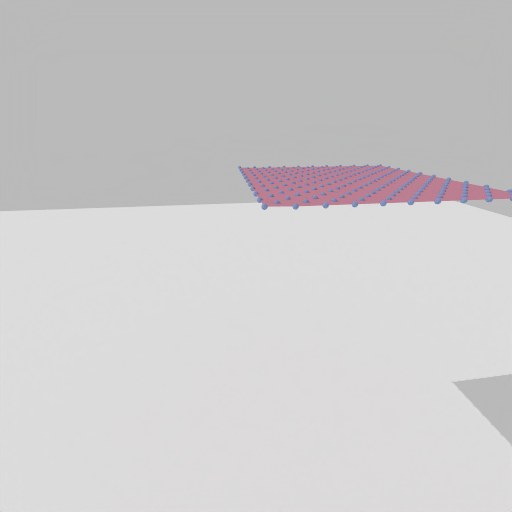
\includegraphics[width=\textwidth]{images/hw0/step_0000.png}
    \end{subfigure}
    \hfill % Add some space between the subfigures
    \begin{subfigure}[b]{0.15\textwidth}
        \centering
        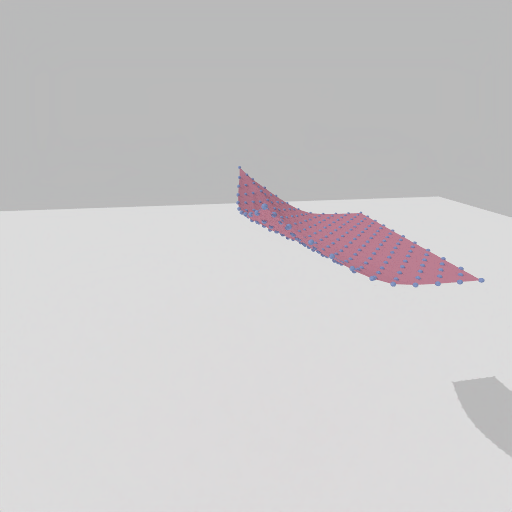
\includegraphics[width=\textwidth]{images/hw0/step_0012.png}
    \end{subfigure}
    \hfill % Add some space between the subfigures
    \begin{subfigure}[b]{0.15\textwidth}
        \centering
        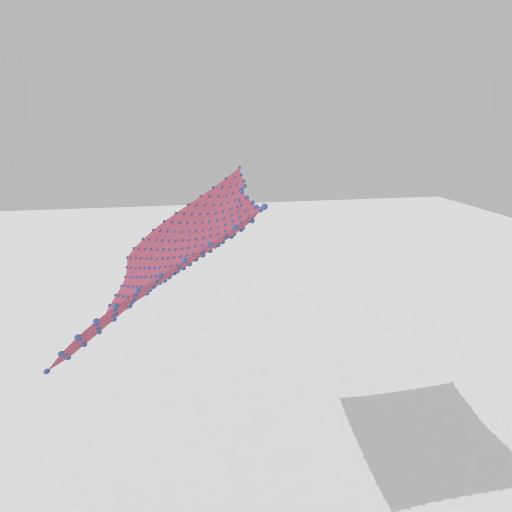
\includegraphics[width=\textwidth]{images/hw0/step_0036.png}
    \end{subfigure}
    \caption{Rendered results.}
    \label{fig:results_frames}
\end{figure}

%%%%%%% -- PAPER CONTENT ENDS -- %%%%%%%%


%%%%%%%%% -- BIB STYLE AND FILE -- %%%%%%%%
\bibliographystyle{IEEEtranS}
\bibliography{refs}
%%%%%%%%%%%%%%%%%%%%%%%%%%%%%%%%%%%%

\end{document}

